\documentclass[tikz,border=8pt]{standalone}
% Shared look for every TikZ diagram. Load with \input{../../tools/tikz-style.tex}
\usepackage[T1]{fontenc}
\usepackage{lmodern}
\renewcommand{\sfdefault}{lmr}  % diagrams use the same serif as the text
\usetikzlibrary{arrows.meta, positioning, shapes.geometric, calc, fit, backgrounds}
\definecolor{cblue}{HTML}{4C78A8}
\definecolor{corange}{HTML}{F58518}
\definecolor{cgreen}{HTML}{54A24B}
\definecolor{cred}{HTML}{E45756}
\definecolor{cpurple}{HTML}{B279A2}
\definecolor{cgrey}{HTML}{6B6B6B}
\tikzset{
  every picture/.style={font=\sffamily, line width=1.2pt},
  box/.style={draw=#1, fill=#1!12, rounded corners=4pt, align=center, inner sep=7pt, minimum height=1.1cm},
  box/.default=cgrey,
  arrow/.style={-{Stealth[length=3mm]}, draw=cgrey, line width=1.4pt},
  title/.style={font=\sffamily\bfseries\Large},
  note/.style={font=\sffamily\small, text=cgrey, align=center},
}
\AtBeginDocument{\hyphenpenalty=10000 \exhyphenpenalty=10000}

\begin{document}
% Section 2: the first record of data/train.json, labelled: an object of key-value pairs, one of whose values is an
% array (ingredients shortened to its first four of nine items).
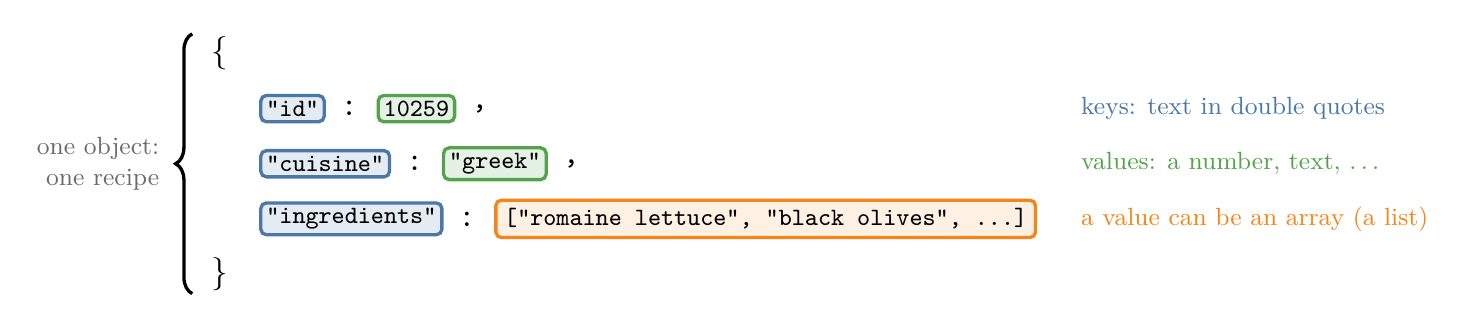
\begin{tikzpicture}[k/.style={draw=cblue, fill=cblue!15, rounded corners=2pt, font=\ttfamily\small, inner sep=2pt},
  v/.style={draw=cgreen, fill=cgreen!15, rounded corners=2pt, font=\ttfamily\small, inner sep=2pt},
  a/.style={draw=corange, fill=corange!12, rounded corners=2pt, font=\ttfamily\small, inner sep=3pt}, t/.style={font=\ttfamily\large}]
  \node[t] (ob) at (0, 0) {\{};
  \node[k, anchor=west] (k1) at (0.5, -0.7) {"id"}; \node[t, right=0.05cm of k1] (c1) {:}; \node[v, right=0.1cm of c1] (v1) {10259}; \node[t, right=0.05cm of v1] {,};
  \node[k, anchor=west] (k2) at (0.5, -1.4) {"cuisine"}; \node[t, right=0.05cm of k2] (c2) {:}; \node[v, right=0.1cm of c2] (v2) {"greek"}; \node[t, right=0.05cm of v2] {,};
  \node[k, anchor=west] (k3) at (0.5, -2.1) {"ingredients"}; \node[t, right=0.05cm of k3] (c3) {:};
  \node[a, right=0.1cm of c3] (v3) {["romaine lettuce", "black olives", \dots]};
  \node[t] at (0, -2.8) {\}};
  \node[note, anchor=west, text=cblue] at (10.8, -0.7) {keys: text in double quotes};
  \node[note, anchor=west, text=cgreen] at (10.8, -1.4) {values: a number, text, \dots};
  \node[note, anchor=west, text=corange] at (10.8, -2.1) {a value can be an array (a list)};
  \draw[decorate, decoration={brace, amplitude=6pt, mirror}] (-0.35, 0.25) -- (-0.35, -3.05) node[midway, left=8pt, note, align=right] {one object:\\one recipe};
\end{tikzpicture}
\end{document}
